\documentclass{article}
\usepackage[utf8]{inputenc}
\usepackage{graphicx}
\usepackage{amsmath }
\usepackage{amssymb}
\usepackage{subcaption}
\usepackage{float}
\usepackage{mathtools}
\setcounter{section}{0}


\usepackage{cleveref} %referencing figures, equations and tables
\crefformat{figure}{Figure.~#2#1#3}
\crefformat{equation}{Eq.~#2#1#3}
\crefformat{table}{Table.~#2#1#3}
\crefformat{appendix}{Appendix.~#2#1#3}
\crefformat{section}{Section.~#2#1#3}

\title{Stadium Truss Static Analysis}
\author{Amir Baharvand }
\date{}

\begin{document}

\maketitle

\section{Problem Statement}
An illustration of a truss, commonly used in stadiums, is provided in \cref{fig:truss_indeterminate}. Prior to modeling, one may notice that the truss is statically indeterminate since node 5 can easily move in the x-direction. The instability of the truss can also be explained through the number of equations and unknowns. Let $e$ be the number of elements and $n$ the number of nodes. The total number of unknowns in the problem is the summation of force in each member ($e$ = 20) and reaction forces at supports (here 3) which becomes 23. The number of equations for a truss in the two-dimension is $2\times n = 2\times 12 = 24$. Therefore, the number of equations is greater than the number of unknowns (24>23). To transform the truss into a statically determinate truss, two approaches may be acquired.

\begin{itemize}
    \item The node 5 $x$-degree-of-freedom should be restrained so that node 5 cannot move along the $x$-axis.
    \item A member should be added between node 1 and node 5.
\end{itemize}

In the following, the first strategy is implemented in the numerical model (see \cref{fig:truss_determinate}). 

\begin{figure}[H]
    \centering
        \begin{subfigure}{0.49\textwidth}
            \includegraphics[width=1\linewidth]{figures/indeterminate.pdf} 
            \caption{The indeterminate truss.}
            \label{fig:truss_indeterminate}
        \end{subfigure}
        \begin{subfigure}{0.49\textwidth}
            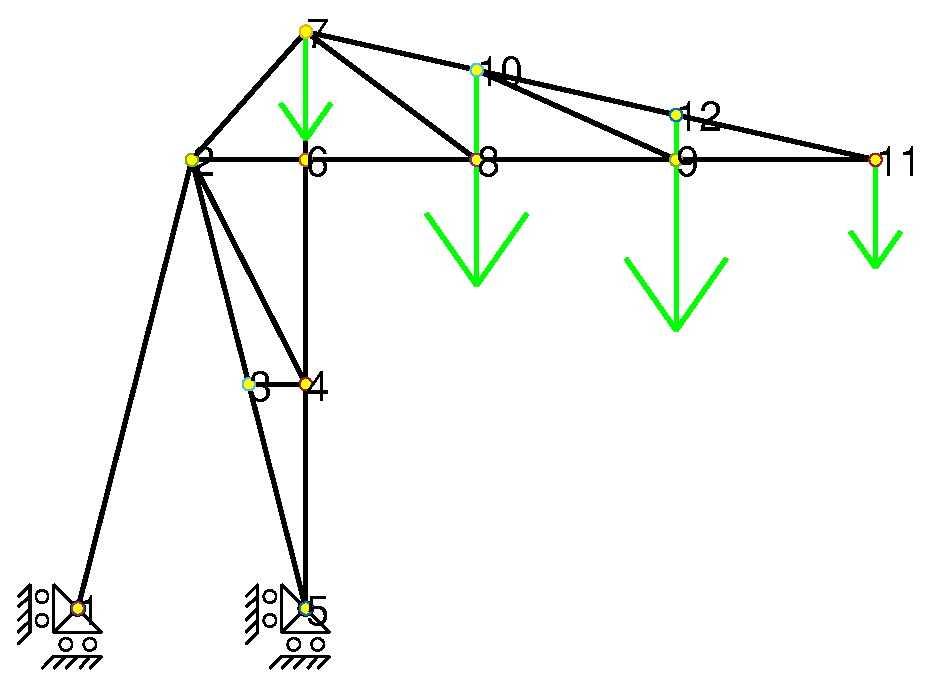
\includegraphics[width=1\linewidth]{figures/determinate.eps} 
            \caption{The determinate truss.}
            \label{fig:truss_determinate}
        \end{subfigure}
    \caption{The geometry, coordinate system and boundary conditions of the truss.}
    \label{fig:truss}
\end{figure}

\section{Numerical Model}
The present problem is modeled as a linear elastic problem due to the absence of contact. In addition, the boundary condition is not a function of time. The displacement is assumed to be infinitesimal and the stress-strain relation follows the Hooke's law.

\subsection{Mechanical Properties}
The numerical model unit is set to SI unit in meter. \cref{tab:mat_prop_truss} summarizes the mechanical properties of the truss members.

\begin{table}[H]
    \centering
    \caption{Mechanical properties of the truss members.}
    \begin{tabular}{l c c c} \hline
        Property & Symbol & Unit & Value \\ \hline
        Young's modulus & $E$& Pa & 2E11 \\
        Poisson's ratio & $\nu$ & - & 0.3 \\
        Area & $A$ & m$^2$ & 1E-02 \\ \hline
    \end{tabular} 
    \label{tab:mat_prop_truss}
\end{table}

\subsection{Solver}
The solver for this problem is set to \textbf{Static, Linear perturbation} because the problem is a static analysis and can be solved within a single step.

\subsection{Mesh Study}
As a truss member is a tow-force member, the stress value all over the length of each member remains constant; hence, each member represents an element.

\subsection{Element Type}
The element type for this problem is T2D2 which is a 2-node linear two-dimensional truss element.

\section{Result and Discussion}
The deformed shape of the truss is given in \cref{fig:truss_displacement}. The blue and red color indicates the members under tension and compression, respectively.


\begin{figure}[H]
    \centering
    \includegraphics[width = 0.6\textwidth ]{figures/truss_displacement.pdf}
    \caption{Unreformed state of the truss (Deformation scale factor=250).}
    \label{fig:truss_displacement}
\end{figure}


%\newpage
%\bibliography{ref}
%\bibliographystyle{ieeetr}

\end{document}